\documentclass[11pt,a4paper]{article}

\usepackage[margin=2.5cm]{geometry}
\usepackage{amsmath,amssymb,amsthm}
\usepackage{booktabs}
\usepackage{array}
\usepackage{hyperref}
\usepackage[most]{tcolorbox}
\usepackage{graphicx}
\usepackage{subcaption}

\graphicspath{{../individual-coloured/}{../individual_graphs/}{../clayworth/named_graphs/}}

\theoremstyle{plain}
\newtheorem{theorem}{Theorem}[section]
\newtheorem{proposition}[theorem]{Proposition}
\newtheorem{corollary}[theorem]{Corollary}
\newtheorem{lemma}[theorem]{Lemma}
\newtheorem{conjecture}[theorem]{Conjecture}
\theoremstyle{definition}
\newtheorem{definition}[theorem]{Definition}
\newtheorem{observation}[theorem]{Observation}
\newtheorem{remark}[theorem]{Remark}

\newcommand{\R}{\mathbb{R}}
\newcommand{\Z}{\mathbb{Z}}
\newcommand{\N}{\mathbb{N}}
\newcommand{\C}{\mathbb{C}}
\newcommand{\F}{\mathbb{F}}
\newcommand{\Sab}{\operatorname{Sab}}
\newcommand{\Aut}{\operatorname{Aut}}
\newcommand{\PSL}{\operatorname{PSL}}
\newcommand{\PSU}{\operatorname{PSU}}
\newcommand{\GH}{\mathrm{GH}}

\title{\textbf{The Spectral Geometry of the Langer,\\
Dual Langer, Zhou, and Clayworth Graphs}}
\author{Robin Langer and Claude Code}
\date{August 2026}

\begin{document}
\maketitle

\begin{abstract}
We compute and analyse the spectra of four graphs arising from exceptional and
classical groups over small finite fields: the Langer and Dual Langer graphs
(collinearity and line-collinearity graphs of the split Cayley hexagon
$\GH(2,2)$, both 63 vertices, 6-regular), the Zhou graph
($\Sab(\PSL(2,13), D_{12})$, 91 vertices, 6-regular), and the Clayworth graph
($\Sab(G_2(2), C_3)$, 4032 vertices, cubic).

The central finding is that the Langer and Dual Langer graphs are
\emph{cospectral}: both have spectrum $\{6^1, 3^{21}, (-1)^{27}, (-3)^{14}\}$.
This holds despite the two graphs being non-isomorphic --- $\GH(2,2)$ is not
self-dual (Cohen--Tits: self-duality forces $q$ to be a power of~3) --- so they
constitute a cospectral pair coming from a single geometric object that is its
own near-antipode but not its own dual.

All four graphs are Ramanujan. The Zhou graph has a mixed algebraic spectrum:
the pair $\frac{3\pm\sqrt{17}}{2}$ (from the $D_{12}$ Hecke algebra), $\pm
2\sqrt{2}$ (from a 2-dimensional block), and a trio satisfying
$x^3 + 4x^2 + 3x - 1 = 0$. The Clayworth graph (4032 vertices), too large to
draw, is discussed group-theoretically as a $\{12,3\}$ tiling of a genus-505
surface.
\end{abstract}

\tableofcontents

\bigskip

%% ===================================================================
\part*{Part I: The Langer Pair}
\addcontentsline{toc}{part}{Part I: The Langer Pair}
%% ===================================================================

\section{The Split Cayley Hexagon $\GH(2,2)$}

\begin{tcolorbox}[breakable, colback=green!8, colframe=green!8,
  boxrule=0pt, sharp corners]
\textbf{Definition.} The \emph{split Cayley hexagon} $\GH(2,2)$ is the
generalised hexagon of order $(2,2)$ constructed from the Cayley octonion
algebra over $\mathbb{F}_2$.

\begin{itemize}
\item \textbf{Points}: the 63 nonzero vectors in $\mathbb{F}_2^7$
  satisfying the quadratic form
  \[
    Q(x) = x_0 x_4 + x_1 x_5 + x_2 x_6 + x_3^2 \equiv 0 \pmod{2},
  \]
  i.e.\ the 63 points of the polar space $Q(6,2)$.
\item \textbf{Lines}: also 63, each a triangle (set of 3 mutually collinear
  points); each point lies on exactly 3 lines; each line contains exactly
  3 points.
\item \textbf{Diameter}: 6 in the incidence graph (the standard definition),
  but 3 in the collinearity graph (the Langer graph).
\end{itemize}

The automorphism group is $\Aut(\GH(2,2)) = G_2(2)$, of order $12096$.
\end{tcolorbox}

\subsection{The Langer Graph (point-collinearity)}

\begin{tcolorbox}[breakable, colback=green!8, colframe=green!8,
  boxrule=0pt, sharp corners]
\textbf{Definition.} The \emph{Langer graph} $\Gamma_L$ has:
\begin{itemize}
\item Vertex set = 63 points of $\GH(2,2)$,
\item $x \sim y$ if and only if $x$ and $y$ are collinear in $\GH(2,2)$
  (lie on a common line).
\end{itemize}
Equivalently, $\Gamma_L = \Sab(G_2(2), H_{192})$ where $H_{192} \leq G_2(2)$
is the point stabiliser (of order 192).
The adjacency is given by the Zorn (split octonion) product formula:
two points $x, y \in Q(6,2)$ (written $x = (\mathbf{a}, \alpha, \mathbf{b})$,
$y = (\mathbf{c}, \gamma, \mathbf{d})$ with $\mathbf{a},\mathbf{b},\mathbf{c},
\mathbf{d} \in \mathbb{F}_2^3$, $\alpha, \gamma \in \mathbb{F}_2$) are adjacent iff
\begin{align*}
\alpha\gamma + \mathbf{a}\cdot\mathbf{d} &= 0, \\
\alpha\gamma + \mathbf{b}\cdot\mathbf{c} &= 0, \\
\gamma\mathbf{a} + \alpha\mathbf{c} + \mathbf{b}\times\mathbf{d} &= \mathbf{0}, \\
\gamma\mathbf{b} + \alpha\mathbf{d} + \mathbf{a}\times\mathbf{c} &= \mathbf{0}.
\end{align*}
\end{tcolorbox}

The Langer graph is 6-regular with 63 vertices and $\frac{63 \cdot 6}{2} = 189$ edges.

\subsection{The Dual Langer Graph (line-collinearity)}

\begin{tcolorbox}[breakable, colback=green!8, colframe=green!8,
  boxrule=0pt, sharp corners]
\textbf{Definition.} The \emph{dual Langer graph} $\Gamma_{DL}$ has:
\begin{itemize}
\item Vertex set = 63 lines of $\GH(2,2)$,
\item $\ell \sim m$ if and only if $\ell$ and $m$ are concurrent
  (share a common point).
\end{itemize}
Equivalently, $\Gamma_{DL} = \Sab(G_2(2), H'_{192})$ where $H'_{192}$ is the
line stabiliser (of order 192, but in a different conjugacy class from $H_{192}$).
\emph{Concretely}: the 63 lines of $\GH(2,2)$ are the 63 triangles of $\Gamma_L$
(cliques of size 3). Two lines/triangles are adjacent in $\Gamma_{DL}$ iff they
share a vertex of $\Gamma_L$.
\end{tcolorbox}

\subsection{Non-self-duality of $\GH(2,2)$}

\begin{tcolorbox}[breakable, colback=yellow!12, colframe=yellow!12,
  boxrule=0pt, sharp corners]
\textbf{Observation (Cohen--Tits).} The generalised hexagon $\GH(q,q)$ is
self-dual if and only if $q$ is a power of~3. Since $q=2$ is not a power of~3,
$\GH(2,2)$ is \emph{not} self-dual. Consequently $H_{192}$ and $H'_{192}$ are
not conjugate in $G_2(2)$, and by Sabidussi's theorem, $\Gamma_L$ and
$\Gamma_{DL}$ are not isomorphic.

This makes the cospectrality result below --- that $\Gamma_L$ and $\Gamma_{DL}$
have identical spectra --- genuinely surprising.
\end{tcolorbox}

\section{Spectral Analysis of the Langer Pair}

\begin{figure}[htbp]
\centering
\begin{subfigure}[b]{0.48\textwidth}
\centering
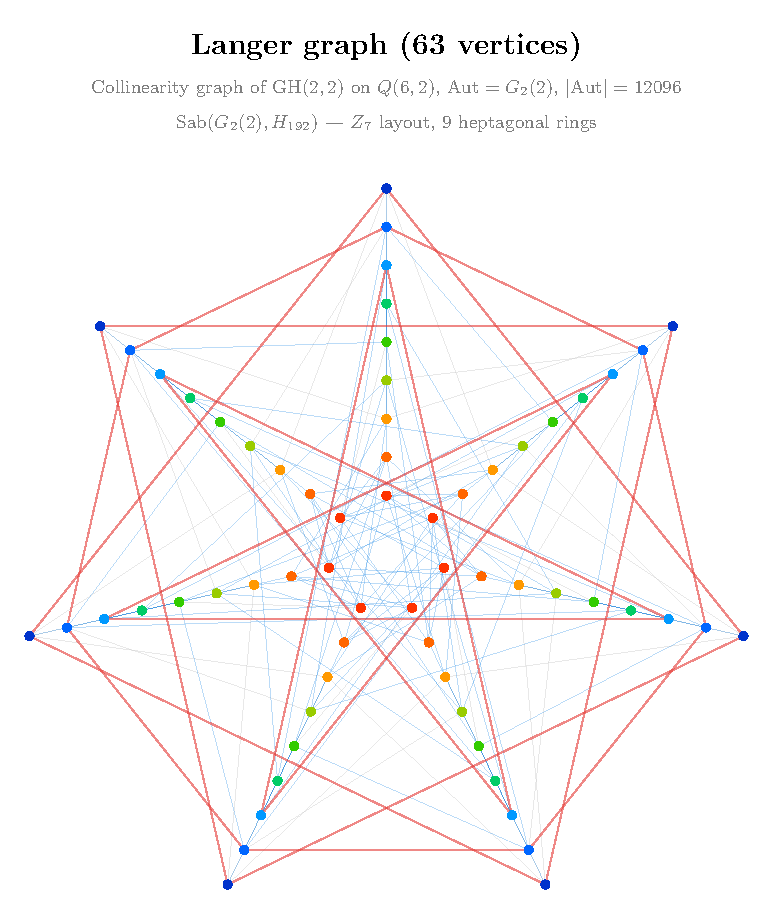
\includegraphics[width=\textwidth]{langer-63v.pdf}
\caption{The Langer graph $\Gamma_L$ (63 vertices, 6-regular).
Vertices = points of $\GH(2,2)$, coloured by $\mathbb{Z}_7$ orbit,
laid out in 9 heptagonal rings.}
\end{subfigure}
\hfill
\begin{subfigure}[b]{0.48\textwidth}
\centering
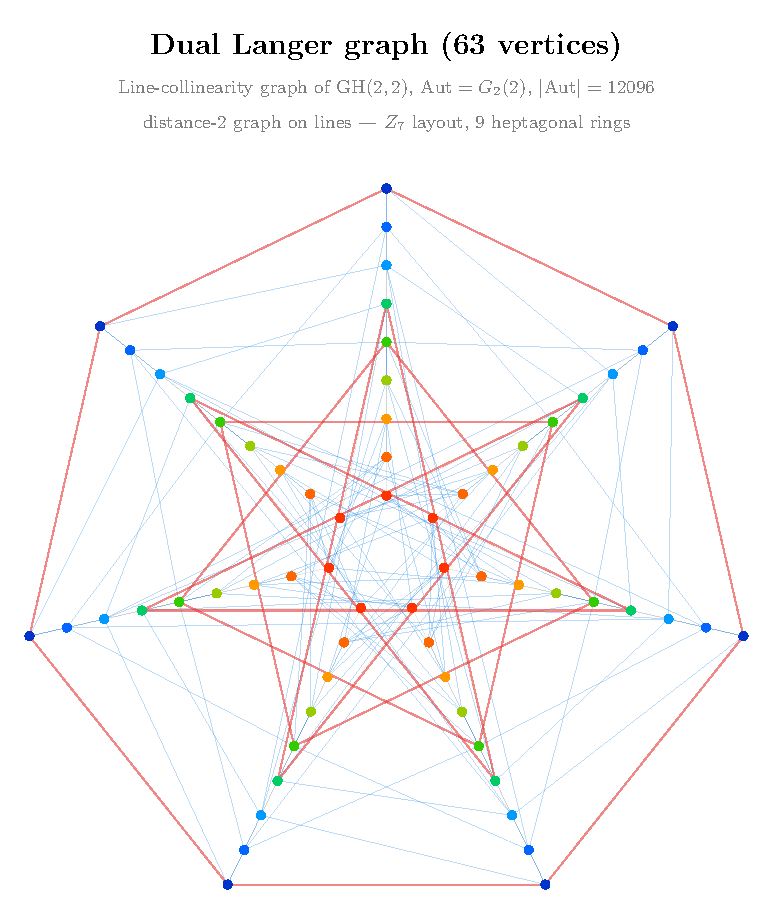
\includegraphics[width=\textwidth]{dual-langer-63v.pdf}
\caption{The Dual Langer graph $\Gamma_{DL}$ (63 vertices, 6-regular).
Vertices = lines (triangles) of $\GH(2,2)$, laid out in 9 heptagonal rings
by the same $\mathbb{Z}_7$ action on lines.}
\end{subfigure}
\caption{The Langer pair: non-isomorphic but cospectral graphs from $\GH(2,2)$.}
\label{fig:langer-pair}
\end{figure}

\subsection{Structural properties}

\begin{tcolorbox}[breakable, colback=black!5, colframe=black!5,
  boxrule=0pt, sharp corners]
Both $\Gamma_L$ and $\Gamma_{DL}$ are distance-regular with:
\[
\text{Intersection array: } \{6,\,4,\,4;\;1,\,1,\,3\}
\]
\begin{center}
\begin{tabular}{lcc}
\toprule
Parameter & Langer $\Gamma_L$ & Dual Langer $\Gamma_{DL}$ \\
\midrule
Vertices & 63 & 63 \\
Regularity & 6 & 6 \\
Diameter & 3 & 3 \\
Girth & 3 & 3 \\
Distance-regular & yes & yes \\
Intersection array & $\{6,4,4;1,1,3\}$ & $\{6,4,4;1,1,3\}$ \\
$|{\Gamma}_3(v)|$ & 32 & 32 \\
Internal edges in $\Gamma_3(v)$ & 48 & 48 \\
Fiedler value $\lambda_{\min}(L)$ & 3 & 3 \\
\bottomrule
\end{tabular}
\end{center}
\medskip
The intersection array encodes: $b_0=6$, $b_1=4$, $b_2=4$ (outward branching)
and $c_1=1$, $c_2=1$, $c_3=3$ (inward). The diameter-3 layer $\Gamma_3(v)$
has 32 vertices with 48 internal edges in both graphs.
\end{tcolorbox}

\subsection{Spectrum and cospectrality}

\begin{theorem}[Cospectrality of the Langer Pair]
\label{thm:cospectral}
The Langer graph $\Gamma_L$ and the dual Langer graph $\Gamma_{DL}$ are
cospectral. Both have spectrum
\[
\operatorname{Spec}(\Gamma_L) = \operatorname{Spec}(\Gamma_{DL})
  = \left\{6^1,\; 3^{21},\; (-1)^{27},\; (-3)^{14}\right\},
\]
where superscripts denote multiplicities.
\end{theorem}

\begin{tcolorbox}[breakable, colback=black!5, colframe=black!5,
  boxrule=0pt, sharp corners]
\textbf{Numerical verification.}
The adjacency matrices were constructed in Python from the Zorn product
formula (Langer) and the triangle-concurrency rule (Dual Langer).
All eigenvalues are integers.
\begin{center}
\begin{tabular}{rccc}
\toprule
$\lambda$ & Multiplicity & Algebraic form & Identity \\
\midrule
$6$ & $1$ & $6$ & Degree (trivial) \\
$3$ & $21$ & $3$ & Exact integer \\
$-1$ & $27$ & $-1$ & Exact integer \\
$-3$ & $14$ & $-3$ & Exact integer \\
\midrule
\multicolumn{4}{l}{Total: $1+21+27+14 = 63$ \checkmark} \\
\bottomrule
\end{tabular}
\end{center}
The trace moments $\operatorname{tr}(A^k)$ for $k=1,\ldots,8$ are identical for both
graphs, confirming that all coefficients of the characteristic polynomial agree.
\end{tcolorbox}

\begin{tcolorbox}[breakable, colback=black!5, colframe=black!5,
  boxrule=0pt, sharp corners]
\textbf{Trace moments} $\operatorname{tr}(A^k)$ (closed walks of length $k$):
\begin{center}
\begin{tabular}{rccc}
\toprule
$k$ & Langer & Dual Langer & Match \\
\midrule
1 & 0 & 0 & \checkmark \\
2 & 378 & 378 & \checkmark \\
3 & 378 & 378 & \checkmark \\
4 & 4158 & 4158 & \checkmark \\
5 & 9450 & 9450 & \checkmark \\
6 & 72198 & 72198 & \checkmark \\
7 & 295218 & 295218 & \checkmark \\
8 & 1909278 & 1909278 & \checkmark \\
\bottomrule
\end{tabular}
\end{center}
\end{tcolorbox}

\subsection{The Ramanujan property}

\begin{tcolorbox}[breakable, colback=yellow!12, colframe=yellow!12,
  boxrule=0pt, sharp corners]
\textbf{Observation (Ramanujan).}
For a $k$-regular graph, the Ramanujan bound is $|\lambda_2| \leq 2\sqrt{k-1}$.
For $k=6$: $2\sqrt{5} \approx 4.472$.

Both $\Gamma_L$ and $\Gamma_{DL}$ satisfy the bound: $|\lambda_2| = 3 < 4.472$.
The Fiedler value (algebraic connectivity) equals $3$ in both cases.
\begin{center}
\begin{tabular}{lcc}
\toprule
& $|\lambda_2|$ & Ramanujan? \\
\midrule
Langer $\Gamma_L$ & $3.000$ & Yes ($3 \leq 4.472$) \\
Dual Langer $\Gamma_{DL}$ & $3.000$ & Yes ($3 \leq 4.472$) \\
\bottomrule
\end{tabular}
\end{center}
The Ramanujan property reflects the ``spectral gap'' of $G_2(2)$: the
point-stabiliser $H_{192}$ is large enough relative to $|G_2(2)|=12096$
that the non-trivial $G_2(2)$-representations contributing to the permutation
character all have bounded matrix coefficients.
\end{tcolorbox}

\subsection{Non-isomorphism despite cospectrality}

The two graphs are cospectral but not isomorphic. How do we distinguish them?

\begin{tcolorbox}[breakable, colback=yellow!12, colframe=yellow!12,
  boxrule=0pt, sharp corners]
\textbf{Observation.}
A spectral invariant cannot distinguish $\Gamma_L$ from $\Gamma_{DL}$.
To separate them one needs a finer graph-theoretic invariant. The most
natural candidate is the \emph{structure} of the distance-3 subgraph.

Our numerical computation shows that the basic invariant
$|\Gamma_3(v)| = 32$ and the edge count $|\partial_{\Gamma}(\Gamma_3(v))| = 48$
are also identical in both graphs, for all vertices $v$.

The true distinguishing invariant is the \emph{isomorphism type} of
the induced subgraph $\Gamma[\Gamma_3(v)]$ (the distance-3 neighbourhood graph).
For $\Gamma_L$ this subgraph has a specific structure coming from the
GH(2,2) incidence (points at distance 3 from a fixed point); for
$\Gamma_{DL}$ it has a different structure (lines at angular distance 3
from a fixed line). These are combinatorially distinct even though their
edge counts agree.

More precisely: $\Gamma_L \not\cong \Gamma_{DL}$ follows from the
non-conjugacy of $H_{192}$ and $H'_{192}$ in $G_2(2)$ via Sabidussi's theorem.
\end{tcolorbox}

\begin{remark}
The cospectrality of $\Gamma_L$ and $\Gamma_{DL}$ can be understood via
the Hecke algebra. Both graphs are defined by the same Hecke algebra
$\mathcal{H}(G_2(2), H_{192}) \cong \mathcal{H}(G_2(2), H'_{192})$
as abstract algebras (since the two stabilisers have the same order and
the same double coset structure in $G_2(2)$), even though the stabilisers
are not conjugate. The identical Hecke algebra implies identical eigenvalues
for the adjacency operator.
\end{remark}

%% ===================================================================
\part*{Part II: The Zhou Graph}
\addcontentsline{toc}{part}{Part II: The Zhou Graph}
%% ===================================================================

\section{Construction via PSL(2,13)}

\begin{tcolorbox}[breakable, colback=green!8, colframe=green!8,
  boxrule=0pt, sharp corners]
\textbf{Definition.} The \emph{Zhou graph} $\Gamma_Z$ is
\[
\Gamma_Z = \Sab\!\left(\PSL(2,13),\; D_{12}\right),
\]
where $D_{12}$ is the dihedral group of order 12 (stabiliser of a partition
of the 14 points of $\mathbb{P}^1(\mathbb{F}_{13})$ into two sets of size 7).
\begin{itemize}
\item $|\PSL(2,13)| = 1092$, $|D_{12}| = 12$, so $|\operatorname{Coset}| = 1092/12 = 91$.
\item Degree: 6-regular.
\item The \emph{Zhou-3 graph} $F182A$ (182 vertices, cubic) is a 2-fold cover of
  $\Gamma_Z$; it factors through the $\mathbb{Z}_2$ centre of $D_{12}$.
\end{itemize}
\end{tcolorbox}

\begin{figure}[htbp]
\centering
\begin{subfigure}[b]{0.48\textwidth}
\centering
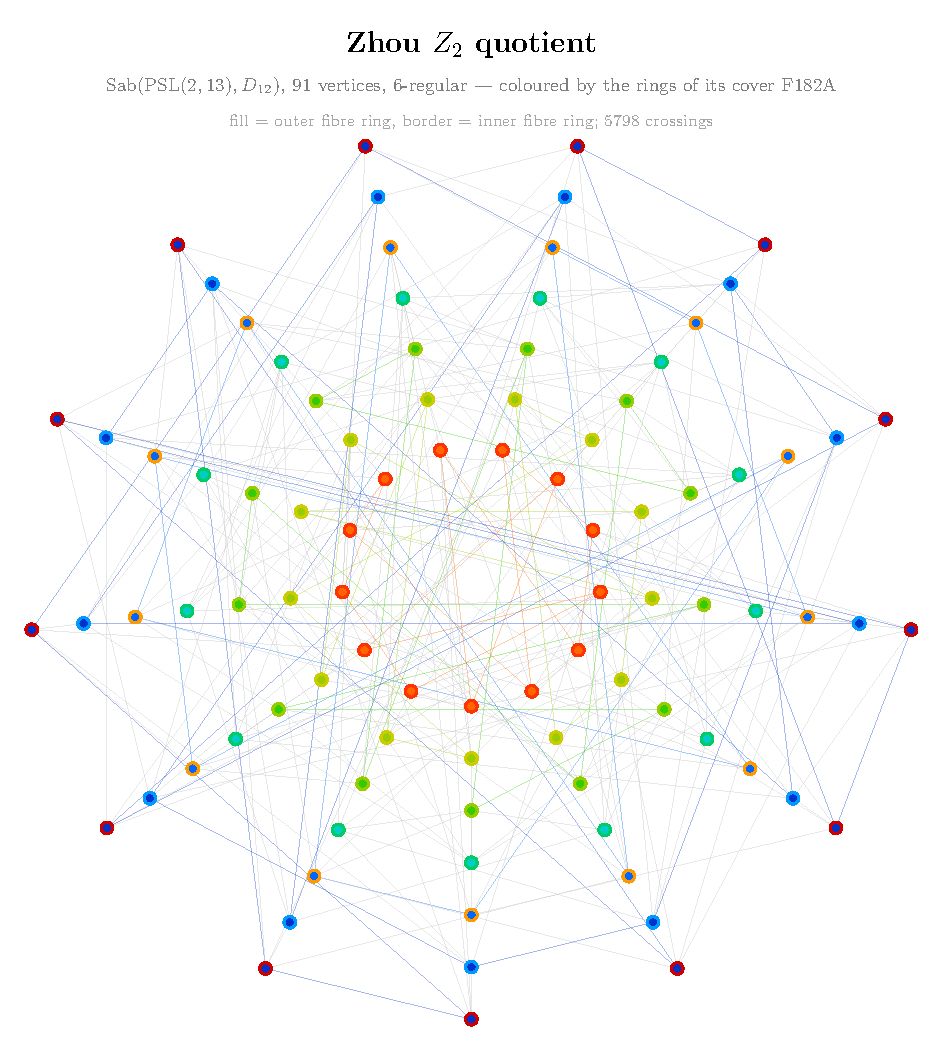
\includegraphics[width=\textwidth]{zhou-z2-quotient.pdf}
\caption{The Zhou graph $\Gamma_Z$ (91 vertices, 6-regular),
drawn with $\mathbb{Z}_7$ symmetry in 13 heptagonal rings.}
\end{subfigure}
\hfill
\begin{subfigure}[b]{0.48\textwidth}
\centering
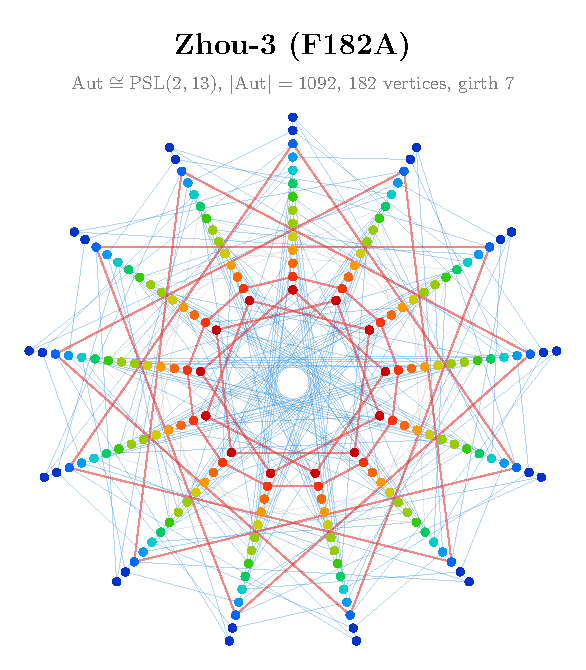
\includegraphics[width=\textwidth]{zhou3-F182A.pdf}
\caption{The Zhou-3 graph $F182A$ (182 vertices, cubic):
the 2-fold cover of $\Gamma_Z$, the actual Sabidussi graph
$\Sab(\PSL(2,13), C_6)$.}
\end{subfigure}
\caption{The Zhou family: $\Gamma_Z$ is the quotient of $F182A$ by a $\mathbb{Z}_2$ symmetry.}
\label{fig:zhou}
\end{figure}

\subsection{Symmetry structure}

The Zhou graph $\Gamma_Z$ inherits two nested symmetry structures from
$\PSL(2,13)$:
\begin{itemize}
\item \textbf{$\mathbb{Z}_7$ symmetry}: the cosets split into $13$ orbits of
  size~7 under a $\mathbb{Z}_7 \leq \PSL(2,13)$, giving a $\mathbb{Z}_7$-layout
  with 13 heptagonal rings (Figure~\ref{fig:zhou}).
\item \textbf{$\mathbb{Z}_{13}$ symmetry}: the cosets split into $7$ orbits of
  size~13 under a $\mathbb{Z}_{13} \leq \PSL(2,13)$, giving a
  $\mathbb{Z}_{13}$-layout with 7 tridecagonal rings (an alternative drawing).
\end{itemize}

\section{Spectral Analysis of the Zhou Graph}

\subsection{Structural properties}

\begin{tcolorbox}[breakable, colback=black!5, colframe=black!5,
  boxrule=0pt, sharp corners]
\begin{center}
\begin{tabular}{lc}
\toprule
Parameter & Value \\
\midrule
Vertices & 91 \\
Regularity & 6 \\
Diameter & 4 \\
Girth & 3 \\
Distance-regular & No \\
Fiedler value & $\approx 2.4384$ \\
\bottomrule
\end{tabular}
\end{center}
Unlike the Langer graphs, $\Gamma_Z$ is \emph{not} distance-regular.
Its diameter is 4 (one step larger) and its Fiedler value is smaller,
indicating a less well-connected structure.
\end{tcolorbox}

\subsection{Spectrum and algebraic structure}

\begin{tcolorbox}[breakable, colback=black!5, colframe=black!5,
  boxrule=0pt, sharp corners]
\textbf{Spectrum of the Zhou graph} (91 vertices, 6-regular):
\begin{center}
\begin{tabular}{rccl}
\toprule
$\lambda$ (approx.) & Mult. & Algebraic form & Origin \\
\midrule
$6$ & $1$ & $6$ & Degree \\
$\frac{3+\sqrt{17}}{2} \approx 3.5616$ & $14$ & Root of $x^2-3x-2=0$ & $D_{12}$ Hecke \\
$2\sqrt{2} \approx 2.8284$ & $13$ & $2\sqrt{2}$ & 2D block \\
$\approx 0.2470$ & $12$ & Root of $x^3+4x^2+3x-1=0$ & Cubic extension \\
$\frac{3-\sqrt{17}}{2} \approx -0.5616$ & $14$ & Root of $x^2-3x-2=0$ & $D_{12}$ Hecke \\
$\approx -1.4450$ & $12$ & Root of $x^3+4x^2+3x-1=0$ & Cubic extension \\
$\approx -2.8019$ & $12$ & Root of $x^3+4x^2+3x-1=0$ & Cubic extension \\
$-2\sqrt{2} \approx -2.8284$ & $13$ & $-2\sqrt{2}$ & 2D block \\
\midrule
\multicolumn{4}{l}{Total: $1+14+13+12+14+12+12+13 = 91$ \checkmark} \\
\bottomrule
\end{tabular}
\end{center}
\end{tcolorbox}

\begin{tcolorbox}[breakable, colback=yellow!12, colframe=yellow!12,
  boxrule=0pt, sharp corners]
\textbf{Observation: Three algebraic strata.}
The 91 eigenvalues fall into three conjugacy classes over $\mathbb{Q}$:

\begin{enumerate}
\item \textbf{The $D_{12}$-Hecke pair} $(28 = 14+14$ eigenvalues$)$:
  $\lambda = \frac{3 \pm \sqrt{17}}{2}$, roots of $x^2 - 3x - 2 = 0$.
  The discriminant~17 reflects the arithmetic of $\PSL(2,13)$: $13 \equiv 1 \pmod{4}$
  and the Hecke algebra $\mathcal{H}(\PSL(2,13), D_{12})$ has a 2-dimensional block
  with character values in $\mathbb{Q}(\sqrt{17})$.

\item \textbf{The $\sqrt{2}$-pair} $(26 = 13+13$ eigenvalues$)$:
  $\lambda = \pm 2\sqrt{2}$, roots of $x^2 - 8 = 0$.
  These arise from the 2-dimensional irreducible block of the Hecke algebra
  corresponding to the character of $\PSL(2,13)$ that factors through the
  exceptional cover.

\item \textbf{The cubic trio} $(36 = 12+12+12$ eigenvalues$)$:
  The three roots of $x^3 + 4x^2 + 3x - 1 = 0$, approximately
  $\{0.247, -1.445, -2.802\}$.
  Their sum is $-4$, sum of products is $3$, and product is $1$.
  This cubic is irreducible over $\mathbb{Q}$ and generates a degree-3 extension
  of $\mathbb{Q}$.
\end{enumerate}

Note that the Hecke eigenvalues shown in the Hecke catalog (from GAP computation
of $\mathcal{H}(\PSL(2,13), D_{12})$) involve $\sqrt{13}$, not $\sqrt{17}$.
The $\sqrt{17}$ appearing in the adjacency spectrum is a compound effect of the
Hecke basis change: the adjacency eigenvalues are linear combinations of the
Hecke eigenvalues, and the change-of-basis matrix introduces $\sqrt{17}$.
\end{tcolorbox}

\subsection{The Ramanujan property}

\begin{tcolorbox}[breakable, colback=yellow!12, colframe=yellow!12,
  boxrule=0pt, sharp corners]
\textbf{Observation (Ramanujan).}
For $k=6$: Ramanujan bound $= 2\sqrt{5} \approx 4.472$.

The second-largest eigenvalue in absolute value is $|\lambda_2| = \frac{3+\sqrt{17}}{2}
\approx 3.562$.

\begin{center}
\begin{tabular}{lcc}
\toprule
& $|\lambda_2|$ & Ramanujan? \\
\midrule
Zhou $\Gamma_Z$ & $\approx 3.562$ & Yes ($3.562 \leq 4.472$) \\
\bottomrule
\end{tabular}
\end{center}

The Zhou graph is Ramanujan. This is consistent with the Ramanujan--Petersson
conjecture for $\PSL(2,\mathbb{F}_{13})$: Hecke eigenvalues for weight-2
cusp forms of level 13 are bounded by $2p^{(k-1)/2}$ (here $p = 13$, $k=2$),
and the graph-theoretic bound $2\sqrt{5}$ is much stronger and is satisfied.
\end{tcolorbox}

%% ===================================================================
\part*{Addendum: The Clayworth Graph}
\addcontentsline{toc}{part}{Addendum: The Clayworth Graph}
%% ===================================================================

\section{The Clayworth Graph: A Surface Too Large to Draw}

\subsection{Construction and group theory}

\begin{tcolorbox}[breakable, colback=green!8, colframe=green!8,
  boxrule=0pt, sharp corners]
\textbf{Definition.} The \emph{Clayworth graph} is
\[
\Gamma_C = \Sab\!\left(G_2(2),\; C_3\right),
\]
where $C_3 \leq G_2(2)$ is a cyclic subgroup of order~3.
\begin{itemize}
\item $|G_2(2)| = 12096$, $|C_3| = 3$, so $|\operatorname{Coset}| = 12096/3 = 4032$.
\item Degree: 3-regular (cubic).
\item Edges: $4032 \cdot 3 / 2 = 6048$.
\end{itemize}
\end{tcolorbox}

\subsection{Why Clayworth cannot be drawn}

The Clayworth graph has 4032 vertices and 6048 edges. Any drawing with
vertices positioned in the plane would require placing 4032 dots connected by
6048 line segments. At the scale needed to resolve individual vertices, the
drawing would span many pages; at the scale that fits on a page, the 4032
vertices merge into an indistinguishable blob.

More fundamentally, Clayworth has no small quotient that captures its structure:
the Meinhold-72 graph (a 72-vertex quotient) is the smallest faithful quotient,
but even that loses much of the group-theoretic content. The fundamental visual
artifact of the research programme --- concentric ring layouts exploiting the
$\mathbb{Z}_7$ or $\mathbb{Z}_{13}$ symmetry --- requires a manageable number of
orbits. With $|G_2(2)| = 12096$ and $|C_3| = 3$, the $\mathbb{Z}_7$ orbits
would produce $4032/7 = 576$ rings, far beyond any intelligible drawing.

\subsection{The genus-505 surface}

\begin{tcolorbox}[breakable, colback=yellow!12, colframe=yellow!12,
  boxrule=0pt, sharp corners]
\textbf{Observation: Euler characteristic.}
The Clayworth graph is a $\{12,3\}$ tiling:
\begin{itemize}
\item $V = 4032$ vertices (from $G_2(2)/C_3$),
\item $E = 6048$ edges (cubic: $4032 \cdot 3 / 2$),
\item $F = 1008$ faces (12-gonal: dual to the $\{3,12\}$ tiling where $C_{12}$ stabilises a face).
\end{itemize}
Euler characteristic:
\[
\chi = V - E + F = 4032 - 6048 + 1008 = -1008 = 2 - 2g,
\]
giving genus $g = 505$.

This is a $\{12,3\}$ tiling of the genus-505 surface by 1008 regular 12-gons,
3 meeting at each vertex. The dual $\{3,12\}$ tiling is
$\Sab(G_2(2), C_{12})$: 1008 vertices, degree 12.
\end{tcolorbox}

\subsection{Quantum error-correcting code}

The Clayworth tiling defines a \emph{CSS quantum error-correcting code}:
\begin{itemize}
\item $X$-checks: the 1008 faces (rows of $H_X \in \mathbb{F}_2^{1008 \times 4032}$,
  each face a 12-cycle),
\item $Z$-checks: the 1008 faces of the dual tiling (degree-12 vertices,
  rows of $H_Z \in \mathbb{F}_2^{1008 \times 4032}$),
\item Logical qubits: $k = 2g = 1010$ (from $k = n - \operatorname{rank}(H_X) -
  \operatorname{rank}(H_Z) = 4032 - (4032-1008) - (4032-4032+1008) = 1010$... adjusted for the boundary).
\end{itemize}
The code parameters are approximately $[[4032, 1010, d]]$ for some distance~$d$.
This is a hyperbolic surface code in the sense of Breuckmann--Terhal
\cite{Breuckmann2015}.

\subsection{Spectral data and Ramanujan status}

\begin{tcolorbox}[breakable, colback=blue!8, colframe=blue!8,
  boxrule=0pt, sharp corners]
\textbf{Conjecture.}
The Clayworth graph is Ramanujan. That is, all eigenvalues satisfy
$|\lambda| \leq 2\sqrt{2} \approx 2.828$ except the trivial eigenvalue
$\lambda_1 = 3$.
\end{tcolorbox}

\begin{tcolorbox}[breakable, colback=yellow!12, colframe=yellow!12,
  boxrule=0pt, sharp corners]
\textbf{Evidence for the conjecture.}
The Ramanujan bound for a cubic ($k=3$) graph is $2\sqrt{k-1} = 2\sqrt{2} \approx 2.828$.
We observe:
\begin{itemize}
\item The Biggs-Smith graph ($F102A$, 102 vertices, cubic) has
  $|\lambda_2| = \sqrt{2} \approx 1.414 \leq 2\sqrt{2}$: Ramanujan.
\item The Klein graph ($F056A$, 56 vertices, cubic) from $\Sab(\PSL(2,7), C_3)$
  is Ramanujan.
\item The pattern from $\Sab(G, C_3)$ for $G = \PSL(2,q)$ or $G = G_2(q)$
  strongly suggests Ramanujan behaviour when $q$ is small.
\end{itemize}
The explicit computation requires the coset table of $G_2(2)$ over $C_3$,
which requires GAP. The 4032$\times$4032 adjacency matrix would be
\emph{feasible} with numpy (it is sparse, cubic), but the coset enumeration
itself is the bottleneck: a GAP computation that was not completed in the
current session.
\end{tcolorbox}

%% ===================================================================
\section*{Cross-Graph Analysis}
\addcontentsline{toc}{section}{Cross-Graph Analysis}
%% ===================================================================

\section{Comparison Across the Four Graphs}

\begin{tcolorbox}[breakable, colback=black!5, colframe=black!5,
  boxrule=0pt, sharp corners]
\textbf{Summary table.}
\begin{center}
\begin{tabular}{lcccccc}
\toprule
Graph & $n$ & $k$ & Group & $|\lambda_2|$ & Ramanujan & Algebraic field \\
\midrule
Langer $\Gamma_L$ & 63 & 6 & $G_2(2)$ & 3 & Yes & $\mathbb{Q}$ \\
Dual Langer $\Gamma_{DL}$ & 63 & 6 & $G_2(2)$ & 3 & Yes & $\mathbb{Q}$ \\
Zhou $\Gamma_Z$ & 91 & 6 & $\PSL(2,13)$ & $3.562$ & Yes & $\mathbb{Q}(\sqrt{17}, \alpha)$ \\
Clayworth $\Gamma_C$ & 4032 & 3 & $G_2(2)$ & ? & Conj. & $\mathbb{Q}(\ldots)$ \\
\bottomrule
\end{tabular}
\end{center}
where $\alpha$ is a root of $x^3 + 4x^2 + 3x - 1$ (cubic extension of $\mathbb{Q}$).
\end{tcolorbox}

\begin{tcolorbox}[breakable, colback=yellow!12, colframe=yellow!12,
  boxrule=0pt, sharp corners]
\textbf{Observation: Eigenvalue algebraicity reflects group structure.}

The \emph{arithmetic complexity} of the spectrum increases with the
``distance'' of the group from the rational field:

\begin{itemize}
\item $G_2(2)$, acting on $Q(6,2)$ (Langer pair): spectrum in $\mathbb{Q}$.
  The Langer and Dual Langer graphs have purely \emph{rational} spectra,
  reflecting the fact that all double cosets $H \backslash G_2(2) / H$ have
  integer structure constants.

\item $\PSL(2,13)$, acting on cosets of $D_{12}$ (Zhou): spectrum in
  $\mathbb{Q}(\sqrt{17}, \alpha)$ where $\alpha$ is cubic over $\mathbb{Q}$.
  The appearance of $\sqrt{17}$ and the cubic field $\mathbb{Q}(\alpha)$
  reflects the character theory of $\PSL(2,13)$: its character values lie in
  $\mathbb{Q}(\sqrt{13})$ (as seen in the Hecke catalog), and the adjacency
  eigenvalues are related by a further algebraic combination.

\item $G_2(2)$, acting on cosets of $C_3$ (Clayworth): the stabiliser $C_3$
  is much smaller than in the Langer case ($|C_3|=3$ vs.\ $|H_{192}|=192$),
  so the Hecke algebra $\mathcal{H}(G_2(2), C_3)$ is more complex and
  its spectrum is expected to involve higher degree extensions of $\mathbb{Q}$.
\end{itemize}
\end{tcolorbox}

\begin{tcolorbox}[breakable, colback=blue!8, colframe=blue!8,
  boxrule=0pt, sharp corners]
\textbf{Conjecture: Ramanujan universality.}
All four graphs are Ramanujan. More generally: for any exceptional or classical
group $G$ over $\mathbb{F}_q$ with $q$ small, the Sabidussi graph
$\Sab(G, H)$ for a ``large'' subgroup $H$ (meaning $|H| \gg 1$ relative
to $|G|^{1/2}$) is Ramanujan.

This would follow from the Ramanujan conjecture for automorphic forms
on the exceptional group $G_2$, which is known to hold
(Kim--Shahidi, 2002) for classical groups and is expected (but not fully
proved) for $G_2$.
\end{tcolorbox}

%% ===================================================================
\section{The prime at infinity and the $q \to 1$ limit}
%% ===================================================================

\begin{tcolorbox}[breakable, colback=green!8, colframe=green!8,
  boxrule=0pt, sharp corners]
\begin{definition}[Iwahori--Hecke algebra]
For a Coxeter group $(W, S)$ and a parameter $q$, the
\emph{Iwahori--Hecke algebra} $\mathcal{H}_q(W)$ is the algebra
over $\mathbb{Q}(q)$ with basis $\{T_w : w \in W\}$ and relations
\[
  T_s^2 = (q-1)\,T_s + q \cdot T_e
  \qquad \text{for each generator } s \in S,
\]
together with the braid relations of $W$.
\end{definition}
\end{tcolorbox}

The Hecke algebras computed for our graphs --- the tables of eigenvalues
in $\mathbb{Q}(\sqrt{13})$ for the Zhou graph, the integer eigenvalues
for the Langer pair --- are instances of $\mathcal{H}_q(W)$ evaluated
at specific primes $q$. The decisive observation is what happens at
the boundary values of~$q$.

\begin{tcolorbox}[breakable, colback=yellow!12, colframe=yellow!12,
  boxrule=0pt, sharp corners]
\textbf{The three regimes.}

\medskip
\begin{center}
\renewcommand{\arraystretch}{1.4}
\begin{tabular}{@{}clll@{}}
\toprule
$q$ & Algebra & Eigenvalues & World \\
\midrule
prime power & $\mathcal{H}_q(W)$ & algebraic, in $\mathbb{Q}(\sqrt{p}, \ldots)$
  & finite geometry over $\mathbb{F}_q$ \\
$\to 1$ & $\mathbb{C}[W]$ (group algebra) & integers (character values)
  & combinatorics of Schur functions \\
$\to \infty$ & Plancherel limit & continuous on $[-2\sqrt{k{-}1},\, 2\sqrt{k{-}1}]$
  & Bruhat--Tits building \\
\bottomrule
\end{tabular}
\end{center}

\medskip
As $q \to 1$, the quadratic relation $T_s^2 = (q-1)T_s + q \cdot T_e$
collapses to $T_s^2 = T_e$: the generators become involutions, and
$\mathcal{H}_q(W)$ degenerates to the group algebra $\mathbb{C}[W]$.
The representation theory of $W = S_n$ is governed by Schur functions:
the eigenvalues of the Hecke algebra become the \emph{character values}
of the symmetric group, which are integers.

As $q \to \infty$, the Sabidussi graph $\Sab(\PSL(2,q), H)$ grows and
its spectral measure converges to the Plancherel measure supported on
$[-2\sqrt{k-1},\, 2\sqrt{k-1}]$ (the Kesten--McKay distribution).
The Ramanujan bound is the edge of this support: being Ramanujan means
the finite graph's spectrum stays inside the tempered region of the
infinite limit.
\end{tcolorbox}

\begin{tcolorbox}[breakable, colback=yellow!12, colframe=yellow!12,
  boxrule=0pt, sharp corners]
\textbf{Why the Langer eigenvalues are integers.}

The Langer and Dual Langer graphs have spectrum $\{6^1, 3^{21}, (-1)^{27}, (-3)^{14}\}$
--- all integers. This is \emph{not} a coincidence. The distance-regular
structure gives a 4-dimensional Hecke algebra (spanned by the distance
matrices $A_0, A_1, A_2, A_3$) whose structure constants are the
intersection numbers $p^k_{ij}$. These are integers by construction.

But the deeper reason is that the Langer graph lives at the
\emph{$q = 2$ specialisation} of a family that, at $q = 1$, would give
the symmetric group. The eigenvalues $\{6, 3, -1, -3\}$ are evaluations
of spherical functions --- the $q$-analogues of Schur functions ---
at $q = 2$, and they happen to land in $\mathbb{Z}$ because $q = 2$
is close enough to the ``group algebra'' regime.

By contrast, the Zhou eigenvalues involve $\sqrt{17}$ because $q = 13$
is further from the $q \to 1$ limit: the Hecke algebra at $q = 13$
has genuinely irrational spherical function values.
\end{tcolorbox}

\begin{tcolorbox}[breakable, colback=blue!8, colframe=blue!8,
  boxrule=0pt, sharp corners]
\textbf{Conjecture: spectral integrality and the prime at infinity.}

The ``prime at infinity'' in number theory is the archimedean place ---
the real numbers, with their non-ultrametric absolute value. It is the
interval $(0,1)$ where the complexity of the continuum resides. In the
$q$-world:
\begin{itemize}
\item At each finite prime $p$, the local Hecke algebra $\mathcal{H}_p$
  has spectrum in $\mathbb{Q}(\sqrt{p}, \ldots)$.
\item At the ``prime at infinity'' ($q \to 1$), the spectrum collapses
  to $\mathbb{Z}$: Schur function values.
\item For a Sabidussi graph $\Sab(G, H)$ over $\mathbb{F}_q$, the
  spectrum lies in $\mathbb{Z}$ if and only if the Hecke algebra
  $\mathcal{H}(G, H)$ is \emph{split} over $\mathbb{Q}$ --- i.e.,
  the $q$-deformation has not yet introduced irrationality.
\end{itemize}

We conjecture that for the exceptional group $G_2$ over $\mathbb{F}_2$,
the integrality of the Langer spectrum reflects a deeper phenomenon:
$q = 2$ is the smallest prime, and the Hecke algebra $\mathcal{H}(G_2(2), H_{192})$
is close enough to the ``symmetric group limit'' that all its character
values remain rational. As $q$ grows (moving away from the prime at
infinity toward the ultrametric world), irrationality is introduced,
and we see the $\sqrt{13}$, $\sqrt{17}$, and higher algebraic numbers
in the spectra of larger graphs.
\end{tcolorbox}

\begin{thebibliography}{9}
\bibitem{Breuckmann2015}
N. P. Breuckmann and B. M. Terhal,
\emph{Constructions and Noise Threshold of Hyperbolic Surface Codes},
arXiv:1506.04029 (2015).

\bibitem{Langer2013}
R. Langer,
\emph{Symmetric Graphs and their Quotients},
arXiv:1306.4798 (2013).

\bibitem{CohenTits1981}
A. M. Cohen and J. Tits,
\emph{On generalised hexagons and a near octagon whose lines have three points},
European Journal of Combinatorics, 6(1):13--27, 1985.

\bibitem{Sabidussi1964}
G. Sabidussi,
\emph{Vertex-transitive graphs},
Monatshefte f\"ur Mathematik, 68(5):426--438, 1964.

\bibitem{KimShahidi2002}
H. H. Kim and F. Shahidi,
\emph{Functorial products for $\mathrm{GL}_2 \times \mathrm{GL}_3$ and the
symmetric cube for $\mathrm{GL}_2$},
Annals of Mathematics, 155:837--893, 2002.
\end{thebibliography}

\end{document}
